\documentclass{beamer}
\usetheme{Boadilla}

\setbeamerfont{block title}{size={}}
\setbeamercolor{titlelike}{parent=structure,bg=white}
\setbeamertemplate{navigation symbols}{}
\usepackage[utf8]{inputenc}
\usepackage{CJK}
\usepackage{verbatim}
\usepackage{graphicx}
\usepackage{multirow}
\hypersetup{CJKbookmarks=true}
\usepackage[T1]{fontenc}
\newcommand{\tabincell}[2]
{
	\begin{tabular}
	{@{}#1@{}}#2
	\end{tabular}
}




\begin{document}
\begin{CJK*}{UTF8}{gkai}
\title{Postgresql Hash} 
\author{马文韬}
\institute{WHU}
\date{\today} 

\frame{\titlepage} 
\frame{\tableofcontents}


\begin{frame}
\transdissolve
\frametitle{存储管理中的哈希}

\begin{figure}[!ht]
\centering
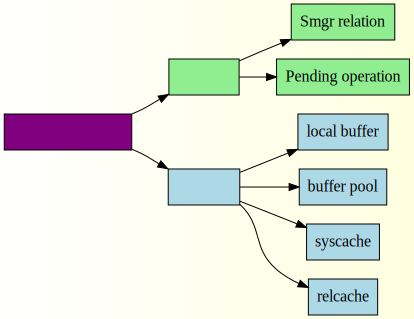
\includegraphics[width = 100mm]{index.jpg}
\caption{存储管理中的哈希图}
\label{overflow}
\end{figure}
\end{frame}

\section{Hash table基本结构及其操作} 
\begin{frame}
\transdissolve
\frametitle{Hash table基本结构图}

\begin{figure}[!ht]
\centering
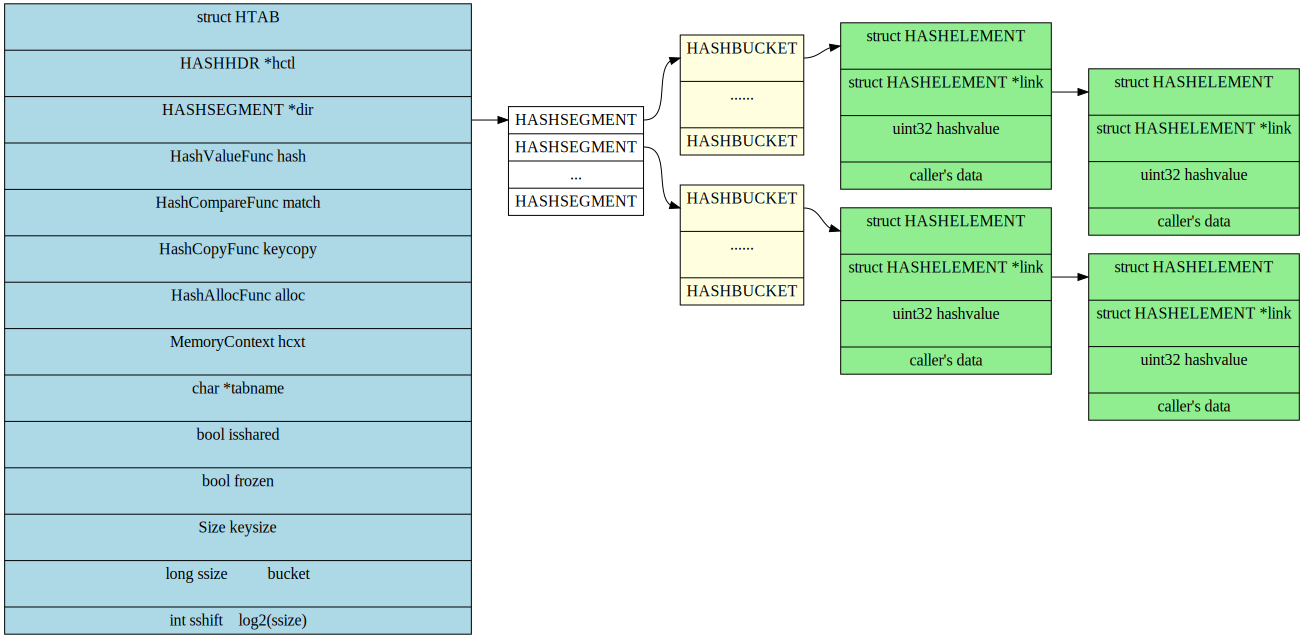
\includegraphics[width = 110mm]{hash.jpg}
\caption{hash table 结构图}
\label{overflow}
\end{figure}
\end{frame}

%\begin{frame}
%\transdissolve
%\frametitle{Hash表相关数据结构}

%\begin{figure}[ht!]
%\begin{tabular}{cc}
%\begin{minipage}[t]{2in}
%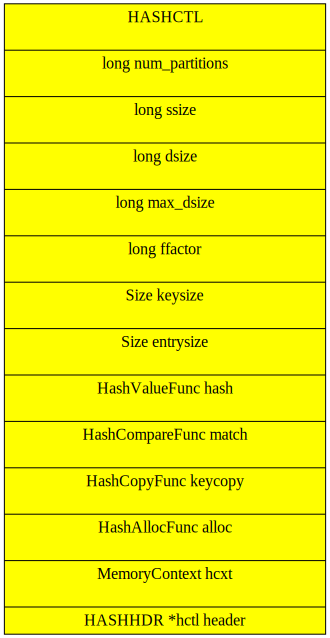
\includegraphics[height = 60mm]{hashctl.jpg}
%\caption{HASHCTL结构图}
%\end{minipage}
%%
%\begin{minipage}[t]{2in}
%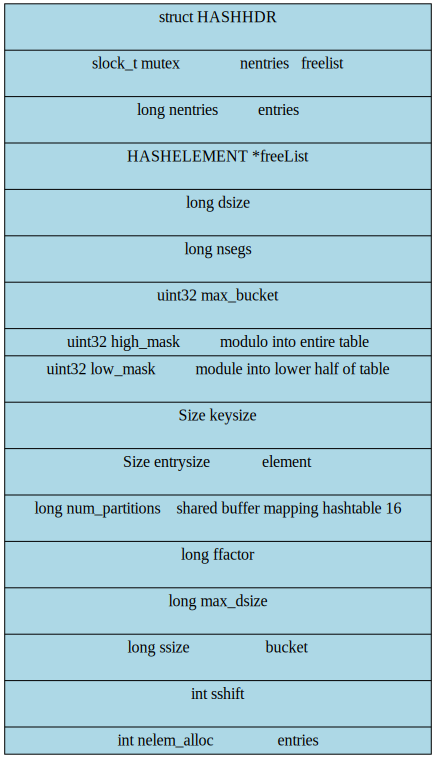
\includegraphics[height = 60mm]{hashhdr.jpg}
%\caption{HASHHDR结构图}
%\end{minipage}
%\end{tabular}
%\end{figure}
%\end{frame}

\begin{frame}
\transdissolve
\frametitle{Hash table基本结构及函数}
%HASHHDR 存在于共享内存中,每个后端还有一个对应的本地HTAB结构,对应非共享哈希表,HASHHDR和HTAB功能上没有区别。\\
\begin{table}
\scriptsize
\centering
\caption{哈希结构体中函数指针的默认函数及其功能}
\label{address}
\begin{tabular}{|c|c|}
\hline
函数指针  &  相关函数 \\
\hline
HashValueFunc hash & 
\tabincell{c}{ string\_hash 计算string哈希值\\tag\_hash 计算tag哈希值\\oid\_hash 计算oid的哈希值\\bitmap\_hash计算bitmap哈希}\\
\hline
HashCompareFunc match & \tabincell{c}{ string\_compare,如果不自定义,默认\\bitmap\_match 和bitmap\_hash一起用}\\
\hline
HashCopyFunc keycopy & \tabincell {c}{strlcpy 可以自定义,默认}\\
\hline
HashAllocFunc alloc  & \tabincell{c}{DynaHashAlloc  调用上下文\\中定义的内存分配方法}\\
\hline
\end{tabular}
\end{table}
\end{frame}


%\begin{frame}
%\transdissolve
%\frametitle{HashValueFunc 类型}
%\begin{table}
%\centering
%\caption{HashValueFucn类型}
%\begin{tabular}{|c|c|}
%\hline
%函数名称  &  函数用途 \\
%\hline
%string\_hash & \tabincell{c}{计算strings的哈希值 }\\
%\hline
%tag\_hash  & \tabincell{c}{计算固定大小\\tag的哈希值}\\
%\hline
%oid\_hash & \tabincell {c}{key是OID,计算哈希}\\
%\hline
%bitmap\_hash & \tabincell{c}{key是bitmap集}\\
%\hline
%bitmap\_match  & \tabincell{c}{和bitmap\_hash一起用,\\用作match函数}\\
%\hline
%\end{tabular}
%\end{table}
%\end{frame}


%\begin{frame}
%\transdissolve
%\frametitle{哈希表相关函数及其操作}
%\begin{table}
%\caption{哈希函数表}
%\begin{tabular}{|c|c|c|}
%\hline 
%函数名 &  主要参数  &  功能 \\
%\hline
%hash\_create & \tabincell{c}{表名,大小,\\HASHCTL结构\\第三个参数标记位} &\tabincell{c}{创建一个动\\态哈希表}\\
%\hline
%hash\_search & \tabincell{c}{哈希表指针,键指针,\\ action标记,\\指向查询结果指针} & \tabincell{c}{对哈希表进行查找,\\插入,删除等操作}\\
%\hline
%\end{tabular}
%\end{table}
%
%\end{frame}

\begin{frame}
\transdissolve
\frametitle{哈希表相关函数及其操作}
\begin{exampleblock}{}
\tiny void *hash\_search(HTAB *hashp,   void *keyPtr,   HASHACTION action,   bool *foundPtr);
\end{exampleblock}
\begin{table}
\caption{hash\_search相关操作action标记}
\begin{tabular}{|c|c|c|}
\hline
 HASH\_FIND & \tabincell{c}{ 根据key\\查找哈希表} \\
\hline
 HASH\_ENTER & \tabincell{c}{ 查找哈希表,\\如果entry没出现,\\那么创建一个 }\\
\hline
 HASH\_ENTER\_NULL & \tabincell{c}{查找哈希表,\\如果超出内存,\\返回NULL}  \\
\hline
 HASH\_REMOVE &\tabincell{c} {移除有特定key的entry} \\
\hline
\end{tabular}
\end{table}
\end{frame}


\section{Smgr relation中的Hash} 
\begin{frame}
\transdissolve
\frametitle{smgr relation中的哈希}
\begin{exampleblock}{RelFileNode}
\tiny
\begin{itemize}
\item \quad Oid spcNode; 表空间
\item \quad Oid dbNode ; 数据库
\item \quad Oid relNode; 关系
\end{itemize}

\end{exampleblock}

\begin{figure}[!ht]
\centering
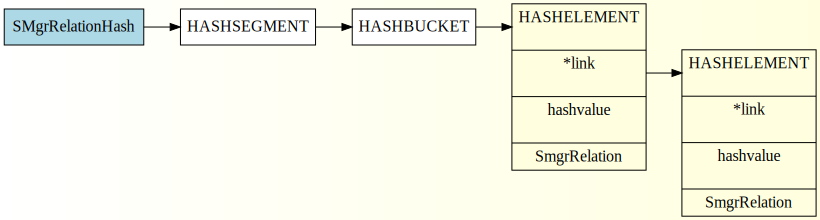
\includegraphics[width = 100mm]{smgr.jpg}
\caption{smgr中的哈希}
\label{overflow}
\end{figure}
\end{frame}


\begin{frame}
\transsplitverticalin
\frametitle{smgr relation中的hash}
\begin{table}
\tiny
\caption{smgr relation中的哈希函数}
\begin{tabular}{|c|c|c|c|}
\hline
\tabincell{c}{函数名}  &
\tabincell{c}{参数}  &
\tabincell{c}{调用函数} &
\tabincell{c}{使用场景}\\
\hline
\tabincell{c}{hash\_search}&
\tabincell{c}{SMgrRelationHash,\\(void *)\&rnode,\\HASH\_ENTER,\&found}&
\tabincell{c}{SMgrRelation  \\smgropen(RelFileNode rnode)}&
\tabincell{c}{RelFileNode作为主键\\查找并返回SMgrRelation对象,\\找不到就创建一个}\\
\hline
\tabincell{c}{hash\_search}&
\tabincell{c}{SMgrRelationHash,\\\&(reln->smgr\_rnode),\\HASH\_REMOVE,NULL}&
\tabincell{c}{void \\smgrclose(SMgrRelation reln)}&
\tabincell{c}{smgr关系的RelFileNode\\作为主键查找并删除\\SMgrRelation对象}\\
\hline
\tabincell{c}{hash\_search}&
\tabincell{c}{SMgrRelationHash,\\(void *)\&rnode\\HASH\_FIND,NULL}&
\tabincell{c}{ void \\smgrclosenode(RelFileNode rnode)}&
\tabincell{c}{RelFileNode作为主键查找返回\\相应SMgrRelation对象,\\由smgrclose完成删除\\避免创建无用关系}\\
\hline
\end{tabular}
\end{table}
\end{frame}


\section{Pending operation中的Hash} 

\begin{frame}
\transdissolve
\frametitle{Pending operation中的哈希}
\begin{columns}
\begin{column}{0.4\textwidth}
\begin{exampleblock}{PendingOperationEntry}
\tiny
\begin{itemize}
\item \quad PendingOperationTag;
\item \quad bool canceled;
\item \quad CycleCtr cycle\_ctr;
\end{itemize}
\end{exampleblock}
\end{column}

\begin{column}{0.4\textwidth}
\begin{exampleblock}{Key:PendingOperationTag}
\tiny
\begin{itemize}
\item \quad RelFileNode rnode;
\item \quad ForkNumber forkNum;
\item \quad BlockNumber  segno;
\end{itemize}
\end{exampleblock}
\end{column}
\end{columns}



\begin{figure}[!ht]
\centering
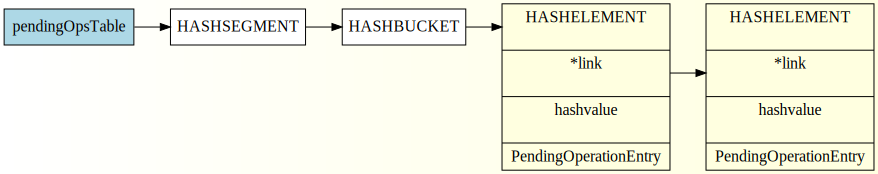
\includegraphics[width = 100mm]{pending.jpg}
\caption{smgr中的哈希}
\label{overflow}
\end{figure}
\end{frame}
\begin{frame}


\transsplitverticalin
\frametitle{pending operation中的hash}
\begin{table}
\tiny
\caption{pending operation中的哈希函数}
\begin{tabular}{|c|c|c|c|}
\hline
\tabincell{c}{函数名}  &
\tabincell{c}{参数}  &
\tabincell{c}{调用函数} &
\tabincell{c}{使用场景}\\
\hline
\tabincell{c}{hash\_search}&
\tabincell{c}{pendingOpsTable,\\\&entry->tag,\\HASH\_REMOVE,\\NULL}&
\tabincell{c}{void mdsync(void)}&
\tabincell{c}{写操作同步到磁盘时\\删除已经无效的操作\\,PendingOperationTag\\作为键查找相应操作并移除}\\
\hline
\tabincell{c}{hash\_search}&
\tabincell{c}{pendingOpsTable,\\\&key,HASH\_ENTER,\\\&found}&
\tabincell{c}{void RememberFsyncRequest\\(RelFileNode rnode,\\ForkNumber forknum,\\BlockNumber segno)}&
\tabincell{c}{PendingOperationTag作为\\主键将fsync的请求\\添加到哈希表中}\\
\hline
\end{tabular}
\end{table}
\end{frame}



\section{SysCache中的Hash} 
\begin{frame}
\transboxout
\frametitle{SysCache 中的Hash}
\begin{figure}[ht!]
\centering
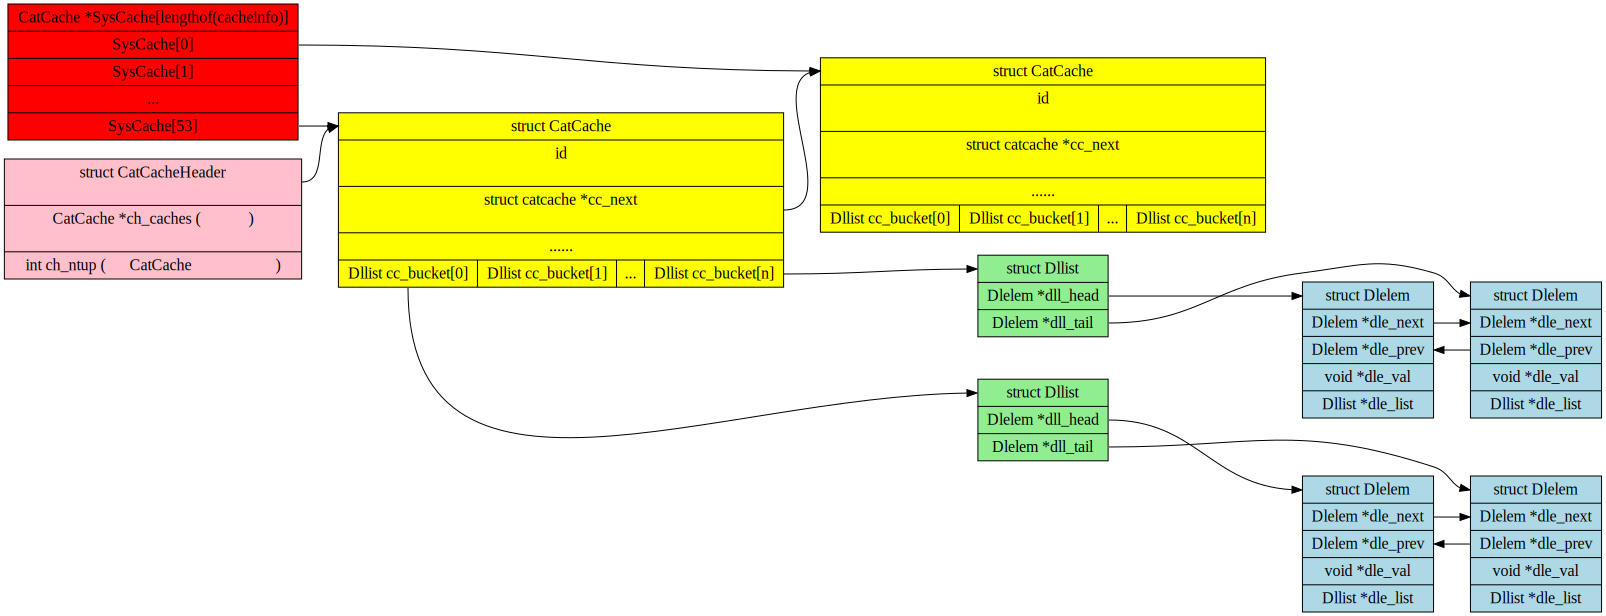
\includegraphics[width = 110mm]{syscache.jpg}
\caption{hash桶结构图}
\label{overflow}
\end{figure}
\end{frame}


\begin{frame}[fragile]
\transboxout
\frametitle{SysCache中的Hash}

\begin{table}
\scriptsize
\caption{精确匹配基本流程及相关函数}
\begin{tabular}{|c|c|}
\hline
初始化关键字信息 & \tabincell{c}{根据四个关键字初始化cur\_skey}\\
\hline
计算哈希值和索引 & \tabincell{c} {CatalogCacheComputeHashValue\\
				由关键字计算hashValue\\
				HASH\_INDEX宏利用hashValue\\
				和cc\_buckets计算索引}\\
\hline
在索引对应的桶中查找 & \tabincell{c}{HeapKeyTest检查key是否匹配\\
				    将匹配的元组移动到链表头}\\
\hline

\end{tabular}
\end{table}
%\end{frame}


%\begin{frame}
%\transboxout
%\frametitle{SysCache中的Hash}
\begin{table}
\scriptsize
\centering
\caption{部分匹配基本流程及相关函数}
\begin{tabular}{|c|c|}
\hline
初始化关键字信息 & \tabincell{c}{根据部分关键字初始化cur\_skey}\\
\hline
计算哈希值和索引 & \tabincell{c} {CatalogCacheComputeHashValue\\
				根据关键字个数计算lhashValue}\\
\hline
\tabincell{c}{在CatCache的cc\_lists\\指向的CatCList链表中查找}         & \tabincell{c}{HeapKey					Test检查key是否匹配\\
		         	将匹配的CatClist放到cc\_lists\\
			 	链表的头部\\
			 	不存在CatCList,扫描物理表并构建}\\
\hline
\end{tabular}
\end{table}
\end{frame}




\section{RelCache中的Hash} 

\begin{frame}
\transdissolve
\frametitle{}
\begin{exampleblock}{Key}
\tiny
Relation 的Oid作为key进行查询。
\end{exampleblock}

\begin{figure}[!ht]
\centering
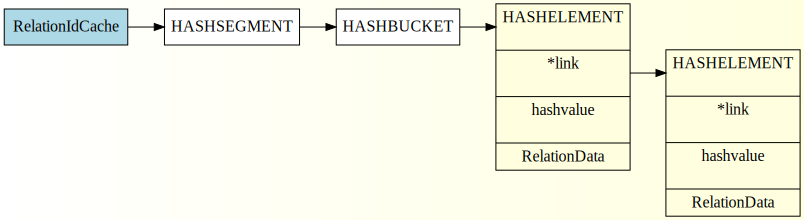
\includegraphics[width = 100mm]{rel.jpg}
\caption{relcache中的哈希}
\label{overflow}
\end{figure}
\end{frame}
\begin{frame}


\transsplitverticalin
\frametitle{RelCache中的hash}
\begin{table}
\tiny
\caption{RelCache中的hash}
\begin{tabular}{|c|c|c|c|}
\hline
\tabincell{c}{函数名}  &
\tabincell{c}{参数}  &
\tabincell{c}{调用宏} &
\tabincell{c}{使用场景}\\
\hline
\tabincell{c}{hash\_search}&
\tabincell{c}{RelationIdCache,\\\&(RELATION->rd\_id),\\HASH\_ENTER\\,\&found}  &
\tabincell{c}{RelationCacheInsert\\(RELATION)} &
\tabincell{c}{以关系的Oid作为\\主键将新的关系\\插入到relcache\\哈希表中}\\
\hline
\tabincell{c}{hash\_search}&
\tabincell{c}{RelationIdCache,\\\&(ID),HASH\_FIND,\\NULL}  &
\tabincell{c}{RelationIdCacheLookup\\(ID,RELATION)}&
\tabincell{c}{用关系Oid作为主键\\在relcache中查找相应对象}\\
\hline
\tabincell{c}{hash\_search}&
\tabincell{c}{RelationIdCache,\\\&(RELATION->rd\_id),\\HASH\_REMOVE,\\NULL}&
\tabincell{c}{RelationCacheDelete\\(RELATION)}&
\tabincell{c}{用关系Oid作为\\主键查找并删除\\relcache相应对象}\\
\hline
\end{tabular}
\end{table}
\end{frame}


%\begin{frame}
%\transsplitverticalin
%\frametitle{共享缓冲区HASH表}
%\begin{table}
%\caption{共享缓冲区内存分配部分}
%\begin{tabular}{|c|c|c|}
%\hline
%\tabincell{c}{函数名}  &
%\tabincell{c}{调用函数} &
%\tabincell{c}{使用场景}\\
%\hline
%\tabincell{c}{hash\_create\\(ENTER)}&
%\tabincell{c}{ShemeInitHash} &
%\tabincell{c}{在共享内存(ShemeIndex)\\中创建并且\\初始化或者追加\\一个哈希表。}\\
%\hline
%\tabincell{c}{hash\_search \\(ENTER\_NULL)}&
%\tabincell{c}{ShmemInitStruct}&
%\tabincell{c}{在共享内存哈希表中初始化\\或者查找一个数据结构}\\
%\hline
%\tabincell{c}{hash\_search \\(REMOVE)}&
%\tabincell{c}{ShmemInitStruct}&
%\tabincell{c}{添加结构时内存溢出,\\移除相应结构}\\
%\hline
%\end{tabular}
%\end{table}
%
%\end{frame}
%



\section{Buffer pool中的Hash} 

\begin{frame}
\transdissolve
\frametitle{smgr relation中的哈希}
\begin{exampleblock}{RelFileNode}
\tiny
\begin{itemize}
\item \quad Oid spcNode; 表空间
\item \quad Oid dbNode ; 数据库
\item \quad Oid relNode; 关系
\end{itemize}

\end{exampleblock}

\begin{figure}[!ht]
\centering
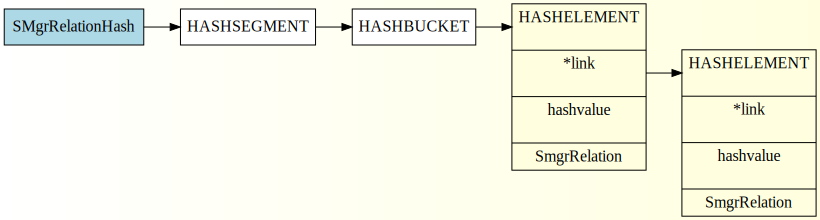
\includegraphics[width = 100mm]{smgr.jpg}
\caption{smgr中的哈希}
\label{overflow}
\end{figure}
\end{frame}



\begin{frame}
\transsplitverticalin
\frametitle{buffer pool 中的hash}
\begin{exampleblock}{BufferTag}
\tiny
rnode(表空间OID,数据库OID和表OID组成);\\
forkNum 枚举类型,标记缓冲区中文件块类型;\\
blockNum  块号
\end{exampleblock}
\begin{table}
\tiny
\caption{buffer pool中的hash}
\begin{tabular}{|c|c|c|c|}
\hline
\tabincell{c}{函数名}  &
\tabincell{c}{参数}  &
\tabincell{c}{调用函数} &
\tabincell{c}{使用场景}\\
\hline
\tabincell{c}{hash\_search\_with\\\_hash\_value}&
\tabincell{c}{SharedBufHash,\\tagPtr,\\hashcode,\\HASH\_FIND,\\NULL}&
\tabincell{c}{int BufTableLookup\\(BufferTag *tagPtr,\\uint32 hashcode)} &
\tabincell{c}{根据BufferTag\\在ShareBufHash中查询,\\返回buffer ID}\\
\hline
\tabincell{c}{hash\_search\_with\\\_hash\_value}&
\tabincell{c}{SharedBufHash,\\tagPtr,\\hashcode,\\HASH\_REMOVE,\\NULL}&
\tabincell{c}{void BufTableDelete\\(BufferTag *tagPtr,uint32 hashcode)}&
\tabincell{c}{根据BufferTag删除\\ShareBufHash中的entry}\\
\hline
\tabincell{c}{hash\_search\_with\\\_hash\_value}&
\tabincell{c}{SharedBufHash,\\tagPtr,\\hashcode,\\HASH\_ENTER,\\\&found}&
\tabincell{c}{int BufTableInsert(BufferTag *tagPtr,\\uint32 hashcode,\\int buf\_id}&
\tabincell{c}{根据BufferTag和\\buffer ID插入entry,\\如果有冲突entry,\\返回冲突entry的buffer ID}\\
\hline
\end{tabular}
\end{table}

\end{frame}



\section{Local buffer中的Hash} 

\begin{frame}
\transdissolve
\frametitle{smgr relation中的哈希}
\begin{exampleblock}{RelFileNode}
\tiny
\begin{itemize}
\item \quad Oid spcNode; 表空间
\item \quad Oid dbNode ; 数据库
\item \quad Oid relNode; 关系
\end{itemize}
\end{exampleblock}
\begin{figure}[!ht]
\centering
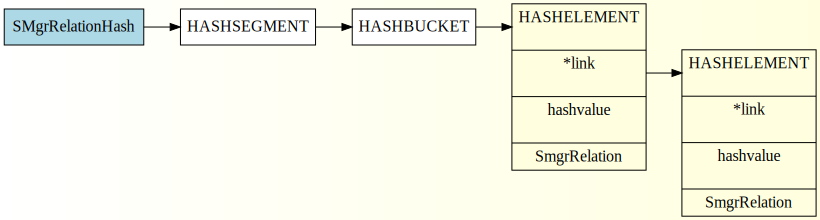
\includegraphics[width = 100mm]{smgr.jpg}
\caption{smgr中的哈希}
\label{overflow}
\end{figure}
\end{frame}

\begin{frame}
\transsplitverticalin
\frametitle{local buffer hash}
\begin{table}
\tiny
\caption{local buffer中的哈希函数}
\begin{tabular}{|c|c|c|c|}
\hline
\tabincell{c}{函数名}  &
\tabincell{c}{参数}  &
\tabincell{c}{调用函数} &
\tabincell{c}{使用场景}\\
\hline
\tabincell{c}{hash\_search}&
\tabincell{c}{LocalBufHash,\&newTag,\\HASH\_FIND,NULL}  &
\tabincell{c}{void LocalPrefetchBuffer\\(SMgrRelation smgr,\\ForkNumber forkNum,\\BlockNumber blockNum)} &
\tabincell{c}{异步读取一个关系块\\用smgr等参数创建一个tag,\\查找LocalBufHash中相应块}\\
\hline
\tabincell{c}{hash\_search}&
\tabincell{c}{LocalBufHash,\&newTag,\\HASH\_FIND,NULL}  &
\tabincell{c}{void LocalBufferAlloc\\(SMgrRelation smgr,\\ForkNumber forkNum,\\BlockNumber blockNum,\\bool *foundPtr)} &
\tabincell{c}{用smgr等参数创建一个tag,\\为给定关系的给定页面创建\\local buffer}\\
\hline
\tabincell{c}{hash\_search}&
\tabincell{c}{LocalBufHash,\\\&bufHdr->tag,\\HASH\_REMOVE,NULL}  &
\tabincell{c}{void LocalBufferAlloc\\(SMgrRelation smgr,\\ForkNumber forkNum,\\BlockNumber blockNum,\\bool *foundPtr)} &
\tabincell{c}{更新LocalBufHash,\\移除旧的entry}\\
\hline
\tabincell{c}{hash\_search}&
\tabincell{c}{LocalBufHash,\\\&bufHdr->tag,\\HASH\_ENTER,NULL}  &
\tabincell{c}{void LocalBufferAlloc\\(SMgrRelation smgr,\\ForkNumber forkNum,\\BlockNumber blockNum,\\bool *foundPtr)} &
\tabincell{c}{更新LocalBufHash,\\创建新的entry}\\
\hline
\end{tabular}
\end{table}

\end{frame}





\end{CJK*}
\end{document}





